\section{Задача 2.12}
\subsection{Задание:}
Вычислить и визуализировать на комплексной плоскости $ \sqrt[5]{4 - 4i} $.
\subsection{Решение:}
$
	\sqrt[5]{4 - 4i}
	=
	\sqrt[5]{4 \sqrt{2} \left( \cos \dfrac{-\pi}{4} - i \sin \dfrac{-\pi}{4} \right)}
	=
	\sqrt[5]{4 \sqrt{2}} \left( \cos \left( \dfrac{-\pi}{4} + \dfrac{2\pi k}{5} \right) -
	i \sin \left( \dfrac{-\pi}{4} + \dfrac{2\pi k}{5} \right) \right), \; k = \overline{0,4}
$
\subsection{Визуализируем в среде Wolfram Mathematica:}
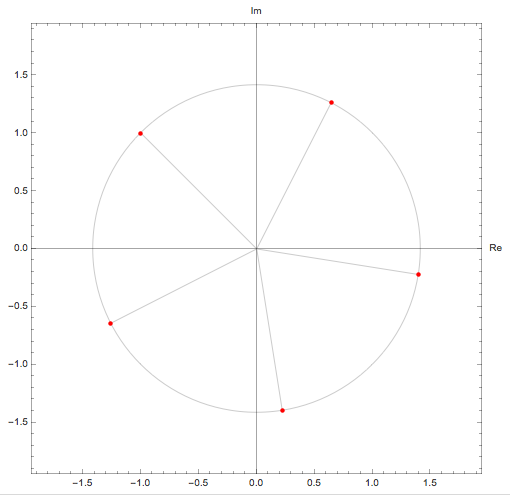
\includegraphics[scale=0.6]{task/2_12/screen.png}
